\subsection{De l'importance de composer les techniques de protection}
\label{fautComposer}

De plus en plus d'applications, en particulier
les applications web et les applications pour téléphone portable,
cherchent à utiliser le nuage, soit pour stocker du code ou des données, 
soit pour faire des calculs,
voir les deux à la fois.

En effet, le cloud peut offrir des services (que ce soit de l'infrastructure,
des plateformes ou du logiciel) disposant d'une forte disponibilité et faciles à redimensionner.

Autrement dit, \emph{pouvoir utiliser le cloud} 
est devenu, dans certains cas,
un enjeu de la conception logicielle,
à cause des avantages de disponibilité 
et redimensionnement que cela offre.

Mais ce n'est pas le seul enjeu de la conception
logicielle.

Vu que la plupart de ces applications manipulent 
des données personnelles, 
garantir la \emph{confidentialité} des données 
est également un enjeu de 
ces applications-là; 
tout comme le sont les \emph{performances} 
pour garantir
une meilleure expérience à l'utilisateur de l'application.

C'est à ces trois enjeux-là de la conception
logicielle (l'utilisation du cloud,
la protection de la confidentialité
et la recherche des performances)
que s'intéresse R. Cherrueau dans sa thèse.

Il s'intéresse également à trois techniques
particulières de protection de la confidentialité
utilisées dans le développement logiciel et regarde comment elles interagissent
avec les trois enjeux cités plus haut.
Ces trois techniques, qu'on va décrire brièvement, sont
	le \emph{chiffrement},
	la \emph{fragmentation verticale} et
	l'\emph{exécution} de l'application \emph{chez l'utilisateur}.

\paragraph{Le chiffrement}
Lorsqu'il est bien utilisé, le chiffrement permet de garantir la confidentialité
des données de l'utilisateur.
De plus, dans certains cas, des calculs peuvent être faits sur les données chiffrées.
On appelle chiffrement homomorphe un chiffrement avec lequel on peut effectuer des calculs
avec les données chiffrées. Les chiffrements homomorphes totaux, comme celui de
Gentry~\cite{gentry:total} sont pour l'instant trop contraignants pour pouvoir être utilisés
dans la plupart des applications, mais les chiffrements homomorphes partiels,
c'est à dire les chiffrements avec lesquels on peut effectuer \emph{certaines}
opérations sur les données chiffrées, peuvent se révéler très utiles.
C'est le cas des chiffrements déterministes (dont les chiffrements symétriques)
qui sont des chiffrements homomorphes partiels, permettant le test d'égalité.

Dans tous les cas, le chiffrement implique un surcoût en terme de calculs,
donc diminue les performances. Dans certains cas, il améliore la confidentialité
et permet l'utilisation du nuage.

\paragraph{L'exécution côté client}
Si le programme était exécuté entièrement par la machine de l'utilisateur,
cela serait à la fois bon pour la confidentialité (car les données
ne seraient pas du tout exposées aux risques liés à l'utilisation du nuage
et du réseau) et pour les performances, puisque, à moins de traiter une 
trop grande quantité de données dans un calcul hautement parallélisable,
les performances du cloud sont moins bonnes que celles des machines des utilisateurs.
Par contre, l'exécution côté client ne permet pas de profiter des avantages du cloud.

\paragraph{La fragmentation verticale} consiste à séparer les différentes données
que manipule le programme entre deux clouds n'ayant aucun rapport entre eux
(à deux endroits géographiques différents, gérés par des entités différentes,
etc$\dots$).
Ceci permet de protéger celles des données personnelles qui sont constituées d'une
\emph{association} de deux données. Par exemple, dans une application stockant
un ensemble de rendez-vous, l'association $\{\mathrm{date}, \mathrm{lieu}\}$
doit être protégée, car une personne malveillante ayant accès à ces deux
informations là à la fois pourrait suivre l'utilisateur de l'application.

L'idée de fragmentation verticale, la façon de l'utiliser,
et même le fait de décrire certaines contraintes de
confidentialité sous la forme d'un couple d'attributs
sont empruntés à un article de 
Aggarwal et al.~\cite{aggar}.

La fragmentation verticale contribue à protéger la confidentialité,
mais d'une façon parfois moins forte que celles du chiffrement
ou de l'exécution côté client. Par contre, chacun des fragments
de données qu'elle génère peuvent être opérés séparément, en introduisant
ainsi, lorsque le programme le permet, une dose de parallélisation
supplémentaire qui peut améliorer les performances et permettre de tirer
encore plus d'avantages du cloud.

\begin{figure}
	\begin{center}
		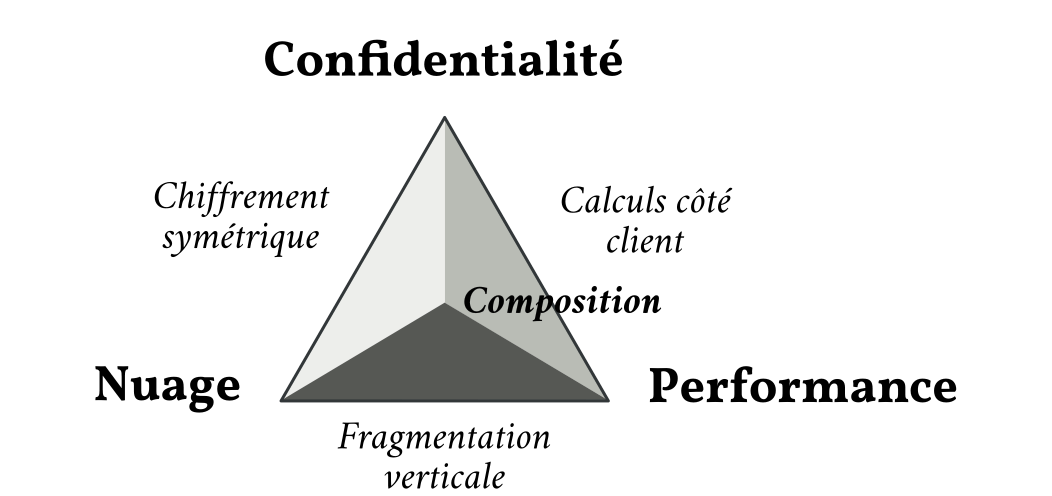
\includegraphics[width=0.7\textwidth]{snps.png}
		\caption{Enjeux et techniques dans le cloud-computing}
		\caption*{(image provenant de la thèse de Ronan Cherrueau~\cite{rc:these})}
		\label{enjeux}
	\end{center}
\end{figure}

La figure \ref{enjeux} résume comment ces trois techniques
là interagissent avec les trois enjeux cités plus haut.

Dans sa thèse, Ronan Cherrueau montre qu'en composant ces différentes techniques
on peut à la fois profiter des avantages du nuage, protéger la confidentialité
et améliorer les performances d'un programme.

Pour pouvoir décrire comment s'effectue une telle composition,
pour pouvoir vérifier la correction d'une telle composition et
pour pouvoir raisonner dessus, Cherrueau a introduit un langage: C2QL.

\subsection{Un langage pour décrire la composition: C2QL}
\label{descrC2QL}
On suppose que l'on peut voir les données stockées par
l'application comme étant une base de données.

Le modèle mathématique le plus répandu pour modéliser
les bases de données est appelé
\emph{algèbre relationnelle}.
Pour une idée plus précise de ce qu'est 
l'algèbre relationnelle, se référer à
la section \ref{defs}, à l'annexe B
ou à la description des fonctions ci-dessous.
L'algèbre relationnelle, comporte, entre
autres, un ensemble de fonctions permettant 
de manipuler les données.

Le langage C2QL donne une façon d'exprimer comment les techniques
mentionnées ci-dessus se composent avec les fonctions classiques de l'algèbre relationnelle.

Les données manipulées sont représentées sous forme de tables, ou relations,
c'est à dire un ensemble de lignes contenant des valeurs pour chacun(e) des 
différent(e)s attributs ou colonnes considéré(e)s.

Dans l'exemple de l'application stockant des rendez-vous, cette
table contiendrait autant de lignes que de rendez-vous stockés 
et (par exemple) trois colonnes ou attributs: 
nom de l'utilisateur
ayant stocké le rendez-vous, date du rendez-vous et lieu du rendez-vous.

\paragraph{Les opérateurs empruntés à l'algèbre relationnelle}
présents dans ce langage sont
\begin{itemize}
	\item La projection, notée $\proj$ 
	qui consiste à ne considérer que certains des attributs de la table (autrement dit,
	à ne garder que certaines colonnes).
	\item La sélection, notée $\sel$
	qui consiste, pour une table donnée, à ne considérer que
	les lignes satisfiant un certain prédicat.
	\item La jonction naturelle, notée $\Join$, qui combine
	les informations de deux tables en fonction des attributs qu'elles ont
	en commun.
	\item L'agrégation et la réduction
	(notées respectivement $\group$ et $\operatorname{fold}$)
	permettant, respectivement, 
	de regrouper les lignes qui partagent les mêmes valeurs
	pour un certain ensemble d'attributs
	et d'effectuer des opérations sur les groupes de lignes ainsi obtenus.
\end{itemize}

\paragraph{Les opérateurs relatifs à la protection des données}
présents dans le langage sont
\begin{itemize}
	\item La fragmentation verticale, notée $\frag$,
	qui sépare une table en deux tables: la première contenant certains
	des attributs (colonnes) de la table d'origine, et la deuxième contenant
	le reste des attributs de la table d'origine.
	
	\item La défragmentation verticale, notée $\defrag$,
	qui effectue l'opération inverse: à partir de deux
	tables n'ayant pas d'attributs en commun, reconstruit une seule table.
	Un attribut spécial, $id$, servant à identifier chaque ligne et conservé lors de 
	la fragmentation d'une table, rend la défragmentation possible.
	
	\item Le chiffrement, noté $\operatorname{crypt}$
	qui chiffre un attribut dans une table.
	
	\item Le déchiffrement, noté $\operatorname{decrypt}$
	qui déchiffre un attribut dans une table.
\end{itemize}

\paragraph{\og Où est passé le calcul côté client?\fg{}}
est une question que vous vous posez peut-être en ce moment.
En effet, il peut paraître étrange que le langage
C2QL n'intégre pas d'opérateur relatif
aux calculs côté client, qui est l'une des techniques
que nous avons annoncée comme étant prise en compte
dans le langage C2QL.

La raison pour laquelle il n'y a aucun opérateur dans C2QL 
qui permette d'exprimer le rapatriement des données sur la machine de l'utilisateur
est liée, d'une part, aux suppositions qu'on fait sur les contraintes
de confidentialité à respecter
(suppositions détaillés plus bas), et,
d'autre part, au fait que
le langage C2QL vise la \emph{sécurité par 
	conception} ou (\emph{security by design}):
le langage doit, dans la mesure du possible,
 être fait de telle façon
qu'un programme écrit dans ce langage soit forcément
sûr.

On suppose, concernant les contraintes de confidentialité
que l'on cherche à respecter, qu'elles sont de l'une des
deux formes suivantes: soit il s'agit du contenu d'un
attribut qu'il faut maintenir confidentiel,
soit c'est l'association entre deux attributs
qu'il faut protéger.

Dans le cas où il faut protéger la confidentialité
d'un seul attribut, le mécanisme utilisé
sera le chiffrement; et donc le fait
de déchiffrer enlève la protection de cet
attribut et implique que, pour que l'application soit
sûre, cette opération de déchiffrement 
et toutes les opérations suivantes doivent être exécutées
sur la machine de l'utilisateur.

Dans le cas où il faut protéger l'association entre deux 
attributs, le mécanisme utilisé
pour protéger cette association est la fragmentation,
et donc toute défragmentation réunissant les deux attributs
en question rompt la protection et nécessite 
que cette défragmentation et les opérations suivantes
soient exécutées sur la machine de l'utilisateur.

% que cette gestion est faite implicitement, pour garantir
%que les requêtes C2QL protègent toujours la confidentialité, par conception.
%En effet, dans le langage C2QL on suppose que les données à protéger sont toujours
%soit un attribut, dans lequel cas il peut être protégé par chiffrement,
%soit une association de deux attributs, dans lequel cas elle peut être protégée
%par fragmentation. Par conséquent, dans une requête, le premier déchiffrement 
%ou la première défragmentation (ou l'absence de chiffrement ou de
%fragmentation dans des cas où ils auraient été nécessaires)
%brisent la protection des données et requièrent que
%les données soient rapatriées chez l'utilisateur pour cette opération et toutes
%les opérations postérieures.

Ainsi, on peut, en regardant une expression C2QL et en connaissant les
contraintes de confidentialité à respecter,
déduire à quel moment les données doivent être rapatriées chez l'utilisateur;
sans que cette opération aie besoin d'apparaître explicitement dans l'expression.
Le rapatriement des données dans la machine de l'utilisateur
est donc gérée implicitement.

%\textbf{Rajouter un exemple serait probablement utile}


Ce langage a été défini comme un Langage de Domaine Spécifique Embarqué dans
Idris. Idris, qui est un langage à types dépendants.
Le système de typage d'Idris et les types donnés aux opérateurs permettent
de vérifier, lorsqu'on écrit une requête en C2QL que celle-ci aura un sens
au moment de l'exécution.

\subsection{Utiliser C2QL: commuter les opérateurs}
\label{passage}
Dans sa thèse, Cherrueau expose une méthode pour se servir facilement
et efficacement de C2QL, en trois étapes.

\paragraph{Première étape: écrire la version locale de l'application.}
Le développeur peut commencer par écrire les requêtes de son application
sans tenir compte de l'utilisation du cloud ni de la protection
des données. C'est ce qu'on appelle ici une version \og locale \fg{}
du programme; c'est le programme tel qu'il pourrait s'exécuter dans la machine de l'utilisateur, localement.
Cette version de l'application est beaucoup plus facile à écrire 
qu'une version utilisant efficacement les techniques de protection.

\paragraph{Deuxième étape: ajouter les techniques de protection nécessaires.}
Comme vu à la section \ref{fautComposer}, le langage C2QL suppose que les contraintes de confidentialité sont de deux types:
soit il s'agit d'une association entre deux attributs que l'on veut 
protéger, et dans ce cas on choisit de mettre les deux attributs de l'association
dans des fragments distincts grâce à la fragmentation verticale, soit il s'agit de la
valeur d'un attribut que l'on veut protéger, et dans ce cas soit on chiffre cette valeur,
soit on la décompose sur plusieurs fragments avec la technique exposée par Aggarwal~\cite{aggar}. Dans les deux cas on peut passer des 
versions locales des requêtes à des versions protégées en faisant apparaître 
à droite de la requête les fonctions de protection composées avec leurs fonctions réciproques.

\paragraph{Troisième étape: faire commuter les différentes fonctions.}
En faisant commuter les différents opérateurs qui apparaissent dans les requêtes,
on peut aboutir à une requête optimisée, profitant des avantages du cloud et de bonnes performances.
Pour cela, on a besoin de savoir à quelles conditions les différents opérateurs de C2QL peuvent
commuter.

C'est sur cet ensemble de lois qui indiquent à quelle condition deux fonctions de C2QL peuvent
commuter que je me suis intéressé pendant mon stage.